% Created 2015-02-01 dom 01:44
\documentclass[xcolor={usenames,svgnames,dvipsnames}]{beamer}
\usepackage[utf8]{inputenc}
\usepackage[T1]{fontenc}
\usepackage{fixltx2e}
\usepackage{graphicx}
\usepackage{longtable}
\usepackage{float}
\usepackage{wrapfig}
\usepackage{rotating}
\usepackage[normalem]{ulem}
\usepackage{amsmath}
\usepackage{textcomp}
\usepackage{marvosym}
\usepackage{wasysym}
\usepackage{amssymb}
\usepackage{hyperref}
\tolerance=1000
\usepackage{color}
\usepackage{listings}
\usepackage{mathpazo}
\usepackage{gensymb}
\usepackage{amsmath}
\bibliographystyle{plain}
\AtBeginSubsection[]{\begin{frame}[plain]\tableofcontents[currentsubsection,sectionstyle=show/shaded,subsectionstyle=show/shaded/hide]\end{frame}}
\AtBeginSection[]{\begin{frame}[plain]\tableofcontents[currentsection,hideallsubsections]\end{frame}}
\usepackage[emulate=units]{siunitx}
\sisetup{per=fraction, fraction=nice, decimalsymbol=comma}
\newunit{\wattpeak}{Wp}
\newunit{\watthour}{Wh}
\newunit{\amperehour}{Ah}
\hypersetup{colorlinks=true, linkcolor=Blue, urlcolor=Blue}
\setbeamercolor{alerted text}{fg=red!50!black} \setbeamerfont{alerted text}{series=\bfseries}
\usetheme[hideothersubsections]{Goettingen}
\usecolortheme{rose}
\usefonttheme{serif}
\author{Oscar Perpiñán Lamigueiro \\ \url{http://oscarperpinan.github.io}}
\date{}
\title{Sistemas Fotovoltaicos Autónomos \\ Componentes}
\hypersetup{
  pdfkeywords={},
  pdfsubject={},
  pdfcreator={Emacs 24.4.1 (Org mode 8.2.7c)}}
\begin{document}

\maketitle

\section{Conceptos Generales}
\label{sec-1}

\begin{frame}[label=sec-1-0-1]{Definición de un Sistema Autónomo}
Un sistema fotovoltaico autónomo (SFA) produce energía eléctrica para \alert{satisfacer el consumo de cargas eléctricas no conectadas a la red}, \alert{empleando un sistema de acumulación energético} para hacer frente a los períodos en los que la generación es inferior al consumo.
\end{frame}

\begin{frame}[label=sec-1-0-2]{Configuracion SHS}
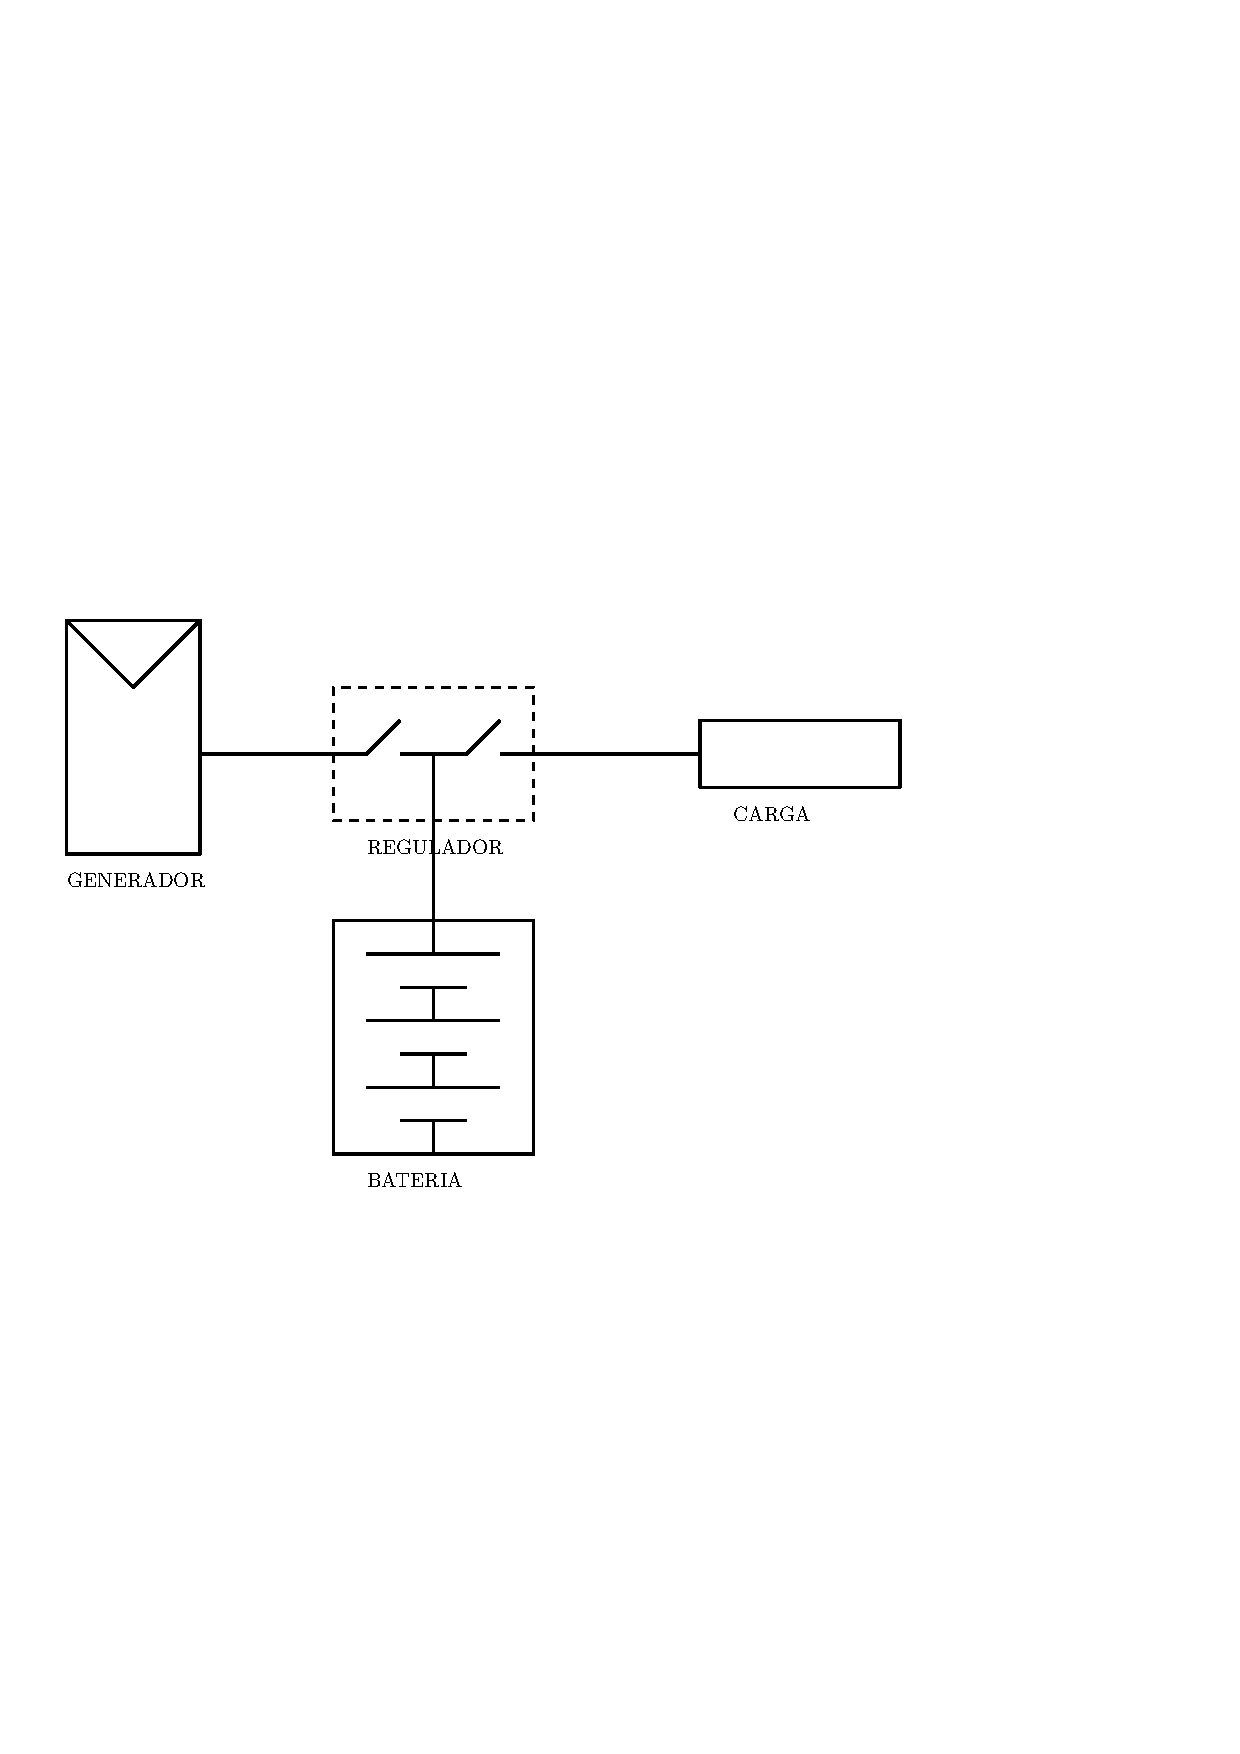
\includegraphics[width=.9\linewidth]{../figs/DiagramaUnifilarER_DC.pdf}
\end{frame}

\begin{frame}[label=sec-1-0-3]{Configuración AC}
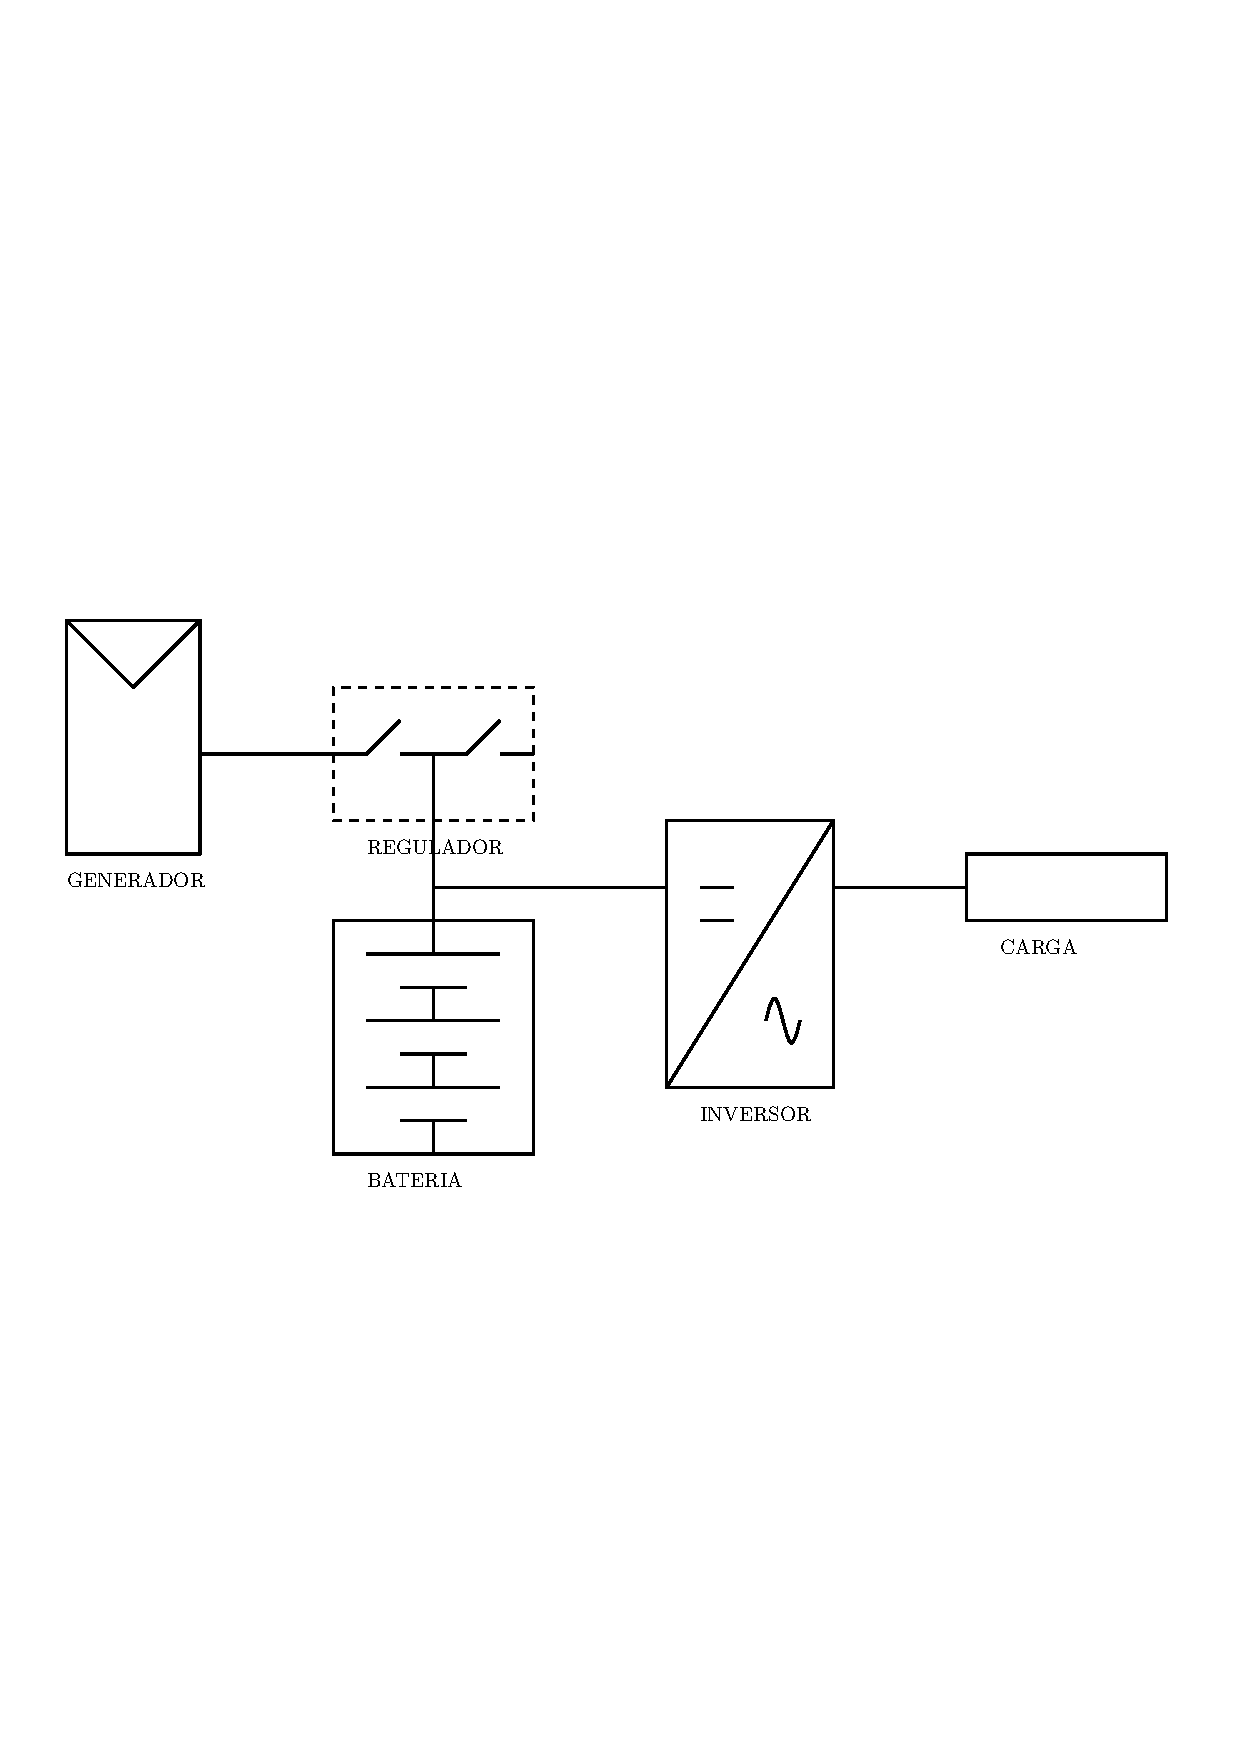
\includegraphics[width=.9\linewidth]{../figs/DiagramaUnifilarER_AC.pdf}
\end{frame}

\begin{frame}[label=sec-1-0-4]{Configuración DC+AC}
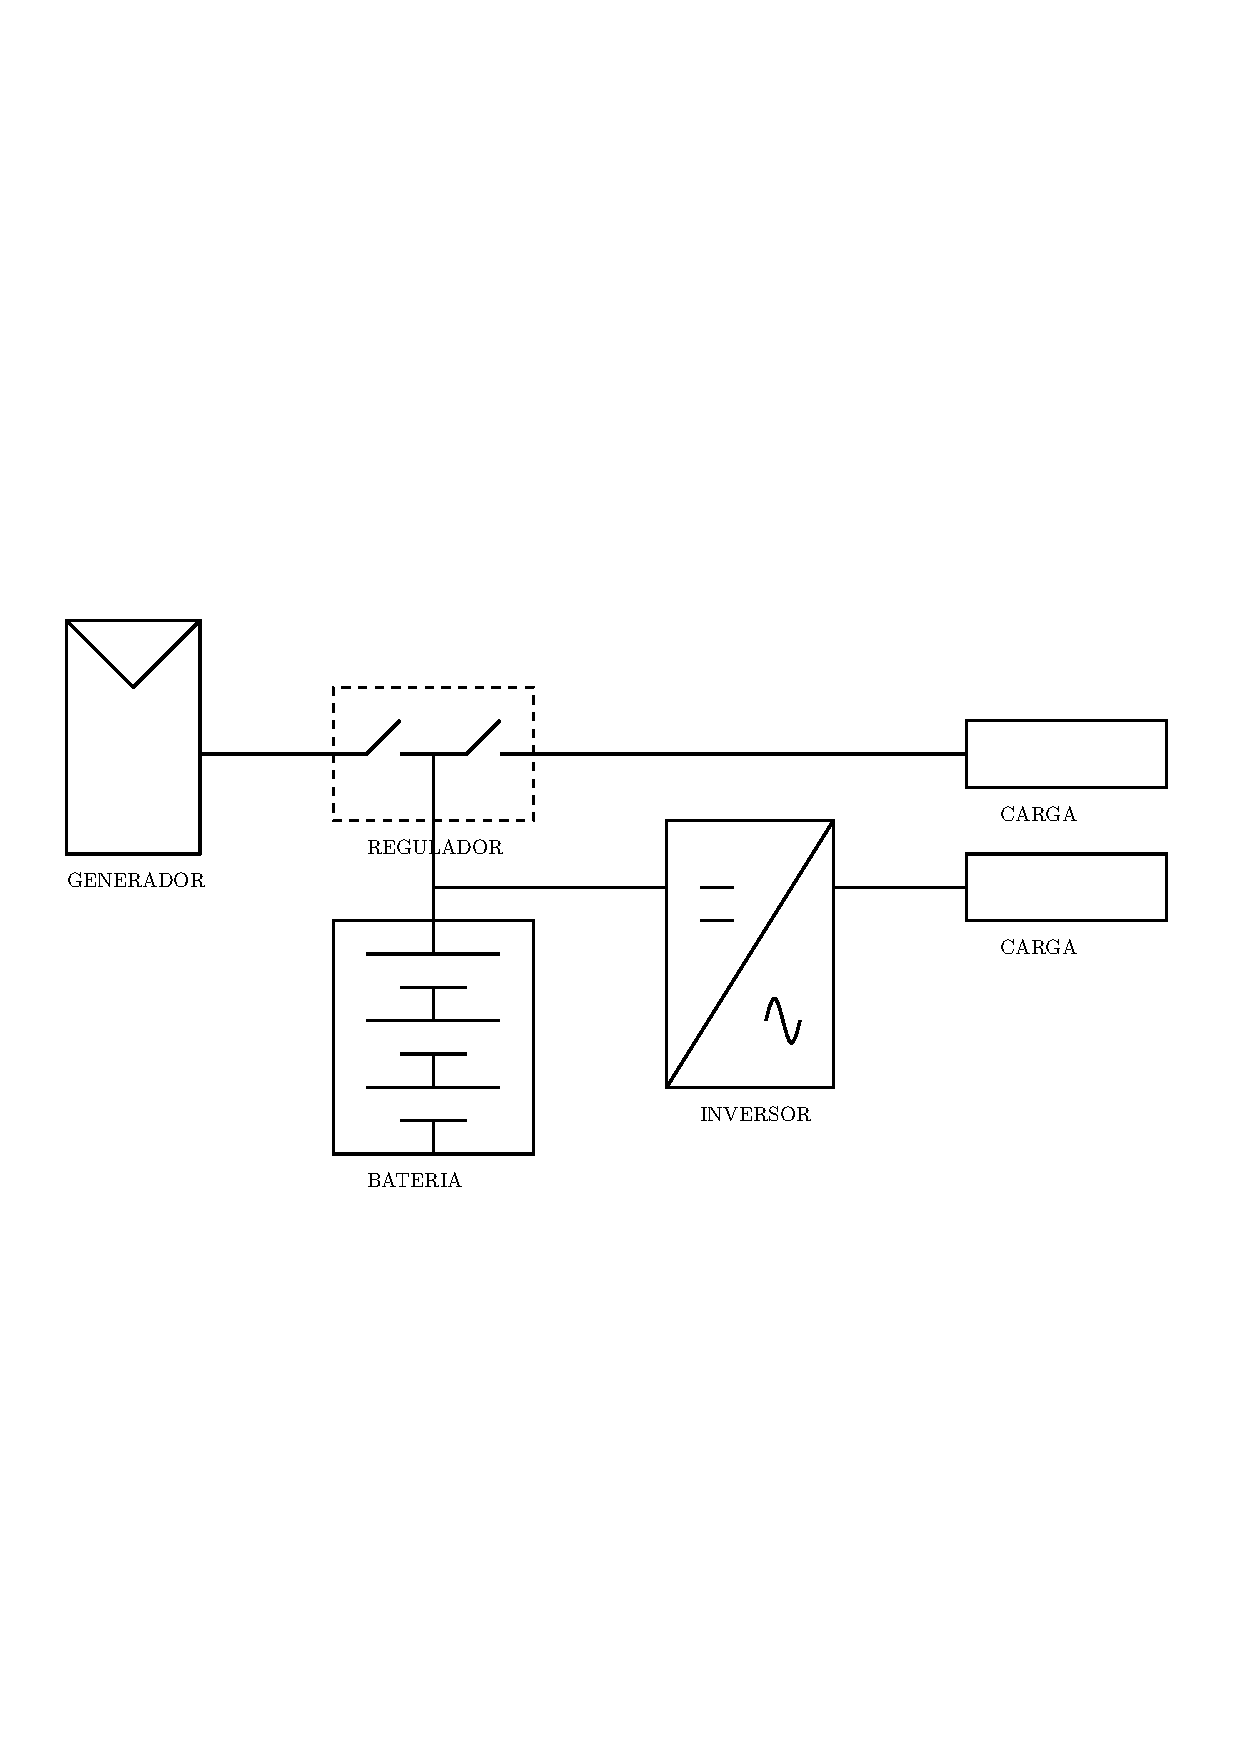
\includegraphics[width=.9\linewidth]{../figs/DiagramaUnifilarER_AC_DC.pdf}
\end{frame}

\begin{frame}[label=sec-1-0-5]{Sistema Híbrido}
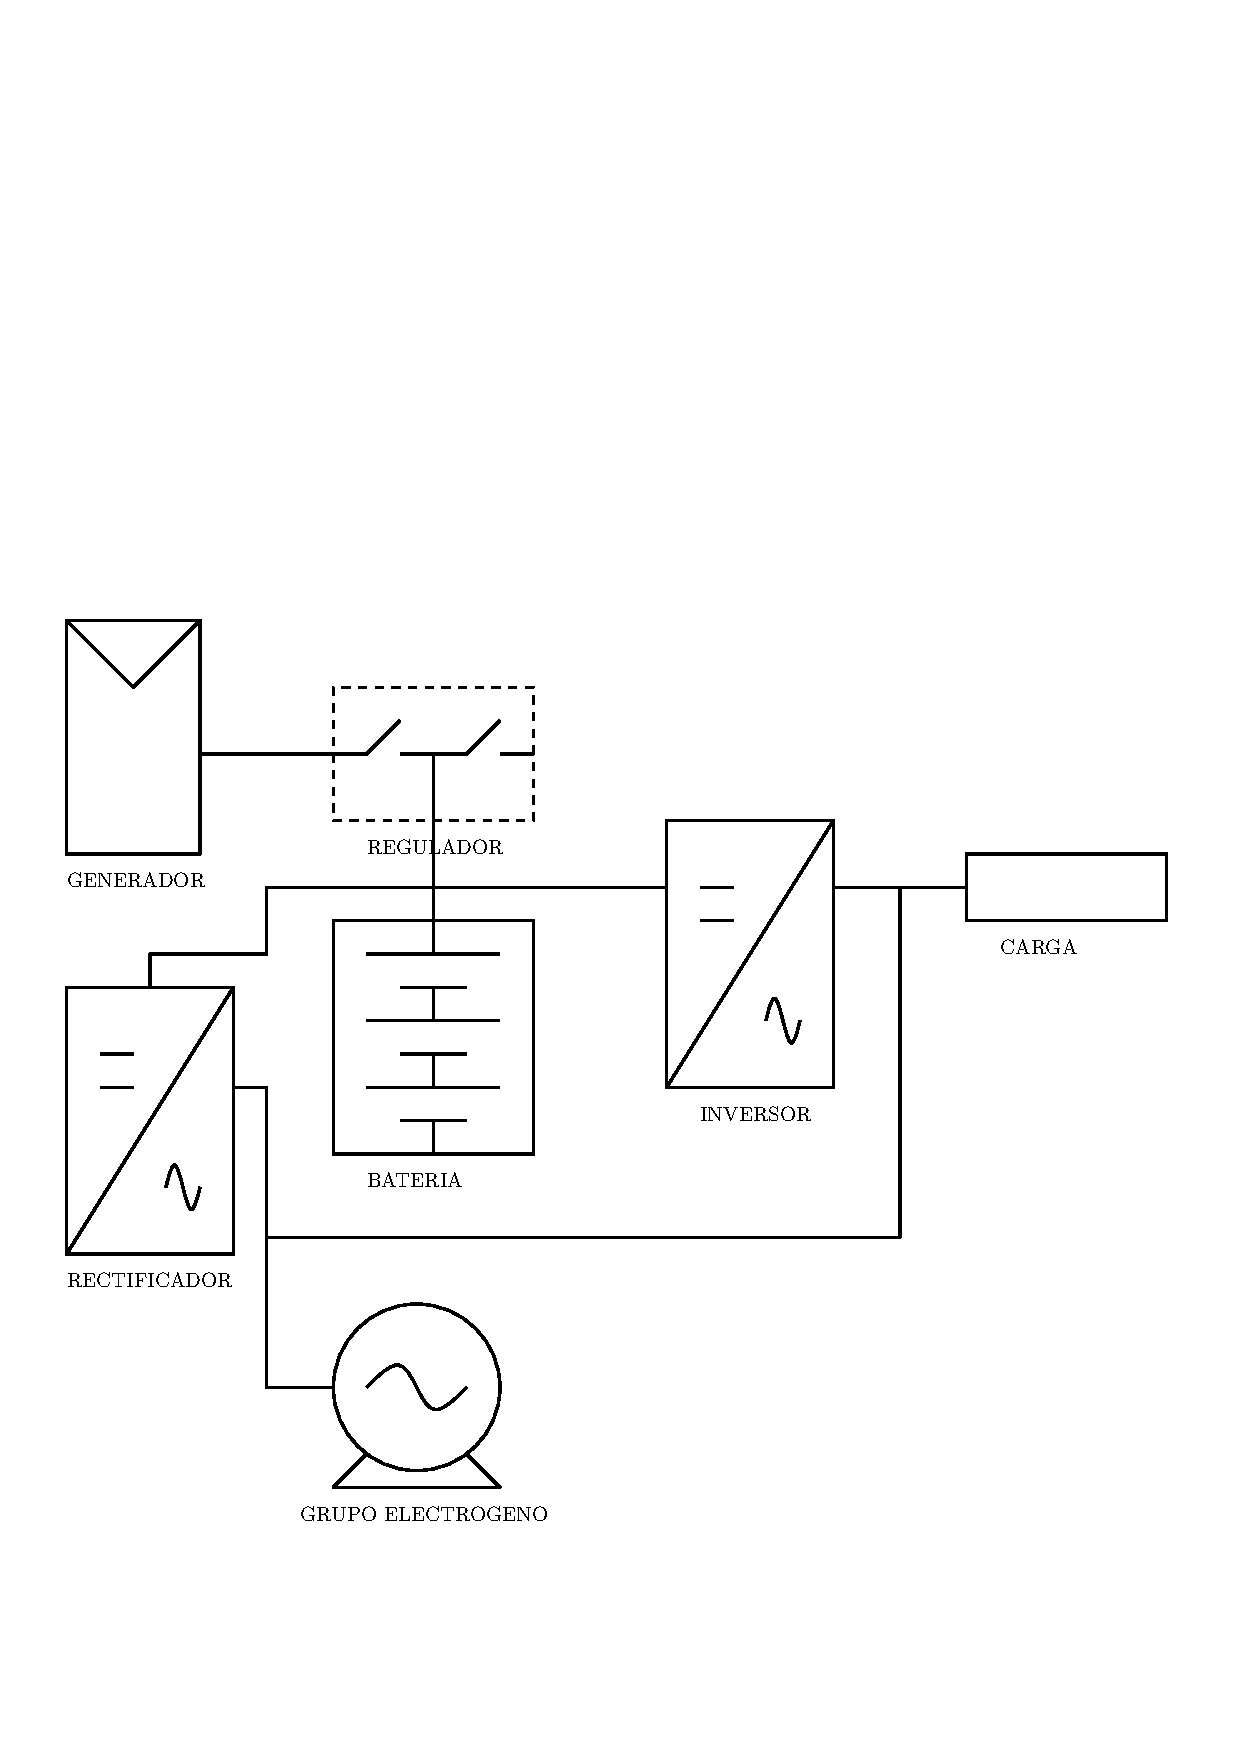
\includegraphics[width=.9\linewidth]{../figs/DiagramaUnifilarER_Hibrido.pdf}
\end{frame}

\section{Acumulador Electroquímico}
\label{sec-2}

\subsection{Definiciones}
\label{sec-2-1}

\begin{frame}[label=sec-2-1-1]{Acumulador electroquímico}
Un acumulador electroquímico es una bateria secundaria o recargable, capaz de almacenar energía eléctrica mediante una transformación en energía electroquímica. Sus principales funciones son:

\begin{itemize}
\item \alert{Autonomía}: satisface los requerimientos de consumo en cualquier momento, independientemente de la generación.

\item \alert{Suministro de picos de intensidad}: cuando es necesario, puede suministrar valores de intensidad superiores a los que proporciona el generador FV.

\item \alert{Estabilización del voltaje}: evita fluctuaciones dañinas para los equipos de consumo.
\end{itemize}
\end{frame}

\begin{frame}[label=sec-2-1-2]{Definiciones}
\begin{description}
\item[{Capacidad nominal ($C_{nom}$)}] es la carga eléctrica que puede ser extraída de una batería hasta llegar a la descarga total.

\item[{Régimen de carga/descarga}] es la corriente aplicada a una batería para restablecer/extraer la capacidad nominal. Normalmente se presenta como un ratio entre la capacidad nominal y la corriente.

\item[{Estado de carga (SoC)}] de una batería es la capacidad de una batería parcialmente cargada, dividida por su capacidad nominal. Por tanto siempre será $0<SoC<1$.
\end{description}
\end{frame}

\begin{frame}[label=sec-2-1-3]{Definiciones}
\begin{description}
\item[{Profundidad de descarga (PD)}] es el complemento del estado de carga.

\item[{Tensión de corte:}] es la tensión a la que finaliza la descarga de la batería. Depende del régimen de descarga y del tipo de batería.  Determina la profundidad de descarga máxima, $PD_{max}$, y por tanto, la capacidad útil, $C_{U}$, siendo $$C_{U}=PD_{max}\cdot C_{nom}$$
\end{description}
\end{frame}

\begin{frame}[label=sec-2-1-4]{Definiciones}
\begin{description}
\item[{Eficiencia farádica}] es el ratio entre la carga extraída durante la descarga y la carga requerida para restablecer el estado inicial.

\item[{Eficiencia energética}] es el ratio entre la energía extraída durante la descarga y la energía requerida para restablecer el estado inicial.
\end{description}
\end{frame}

\subsection{Principios de funcionamiento}
\label{sec-2-2}

\begin{frame}[label=sec-2-2-1]{}
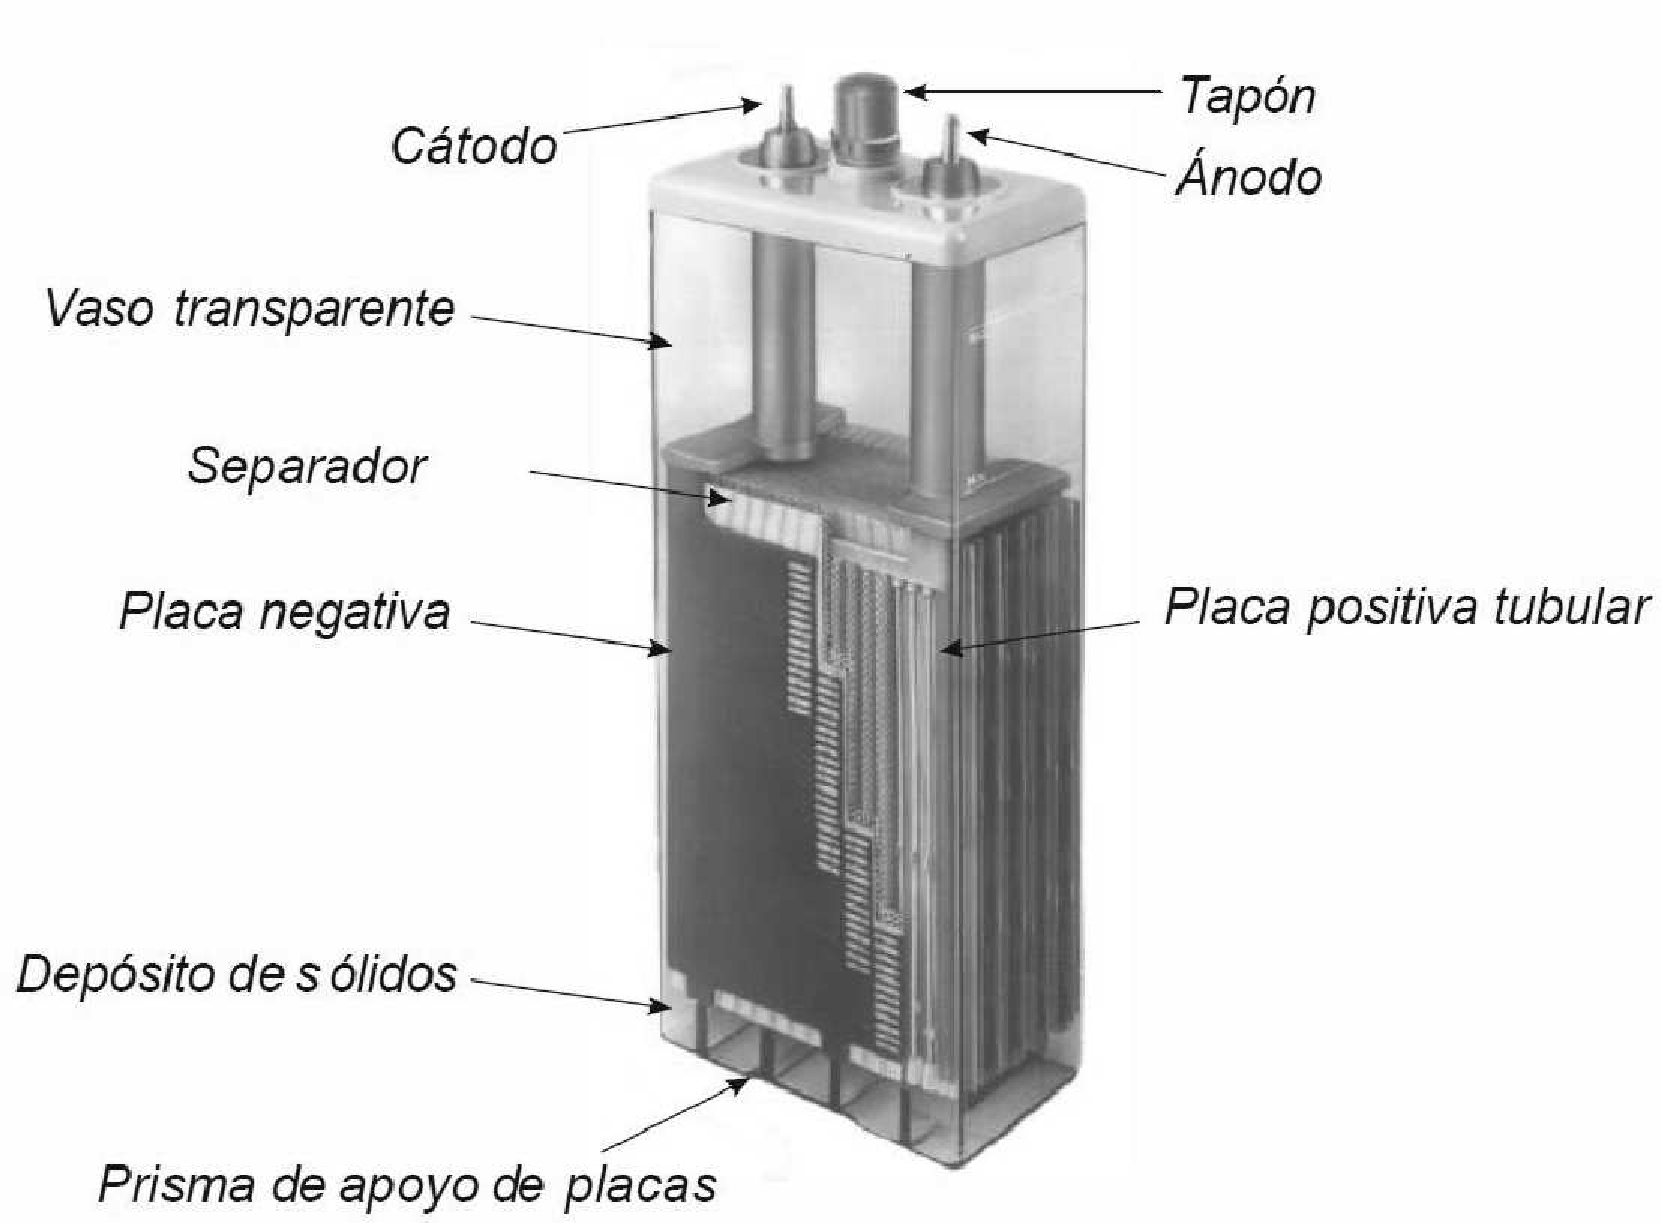
\includegraphics[width=.9\linewidth]{../figs/AcumuladorBN.pdf}
\end{frame}

\begin{frame}[label=sec-2-2-2]{Principios de funcionamiento}
Una batería de ácido-plomo se compone de:

\begin{itemize}
\item Un \alert{ánodo o electrodo positivo} con PbO$_{\text{2}}$

\item Un \alert{cátodo o electrodo negativo} con Pb.

\item \alert{Electrolito} a base de $H_{2}SO_{4}$ diluido en agua.
\end{itemize}
\end{frame}


\begin{frame}[label=sec-2-2-3]{Principio de funcionamiento}
\begin{itemize}
\item Ánodo (+)
\end{itemize}
$$\mathrm{PbO_{2}+SO_{4}^{2-}+H^{+}+2e^{-}\rightleftarrows PbSO_{4}+2H_{2}O}$$

\begin{itemize}
\item Cátodo (-)
\end{itemize}
$$\mathrm{Pb+SO_{4}^{2-}\rightleftarrows PbSO_{4}+2e^{-}}$$

\begin{itemize}
\item Global
\end{itemize}
$$\mathrm{Pb+PbO_{2}+2H_{2}SO_{4}\rightleftarrows2PbSO_{4}+2H_{2}O}$$
\end{frame}

\begin{frame}[label=sec-2-2-4]{Evolución de la tensión en un proceso de carga}
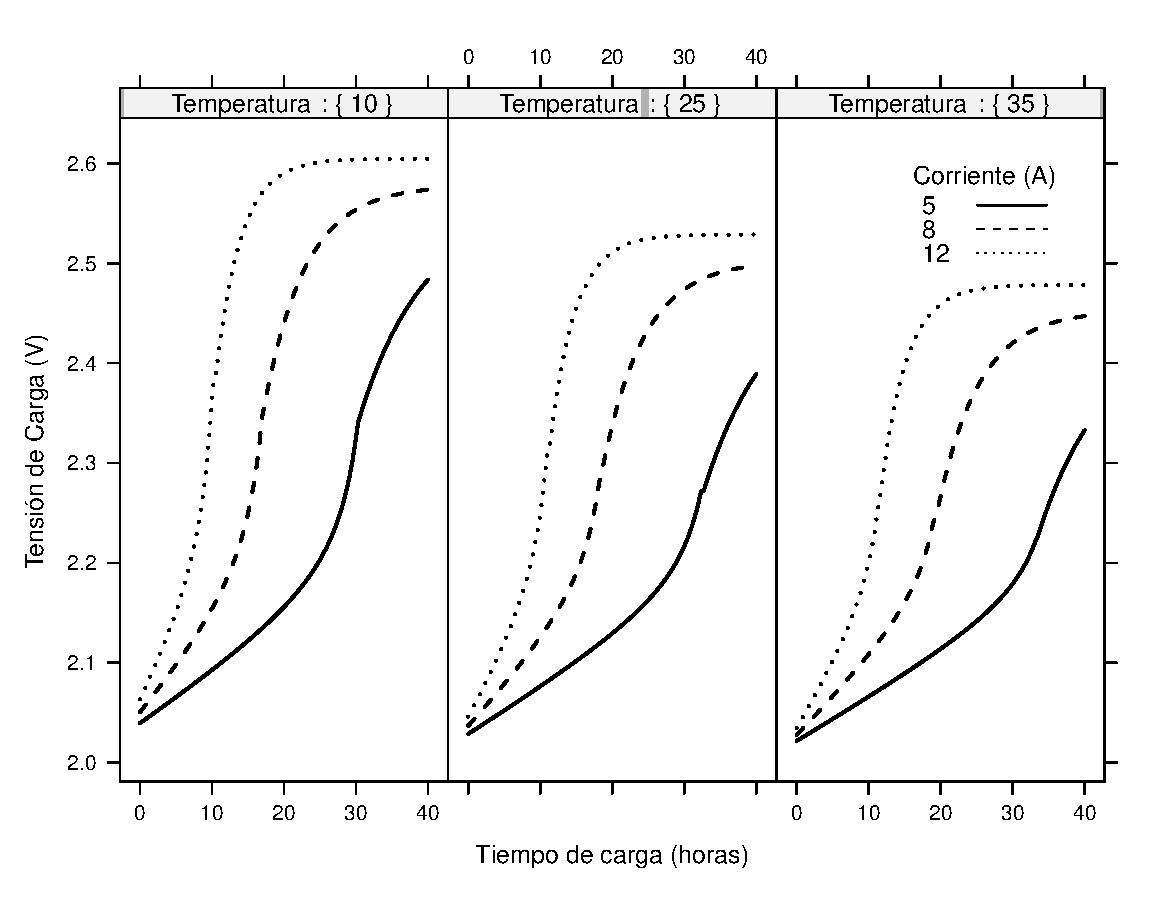
\includegraphics[width=.9\linewidth]{../figs/Bateria_CorrYTemp.pdf}
\end{frame}

\begin{frame}[label=sec-2-2-5]{Evolución de la tensión durante un proceso de descarga}
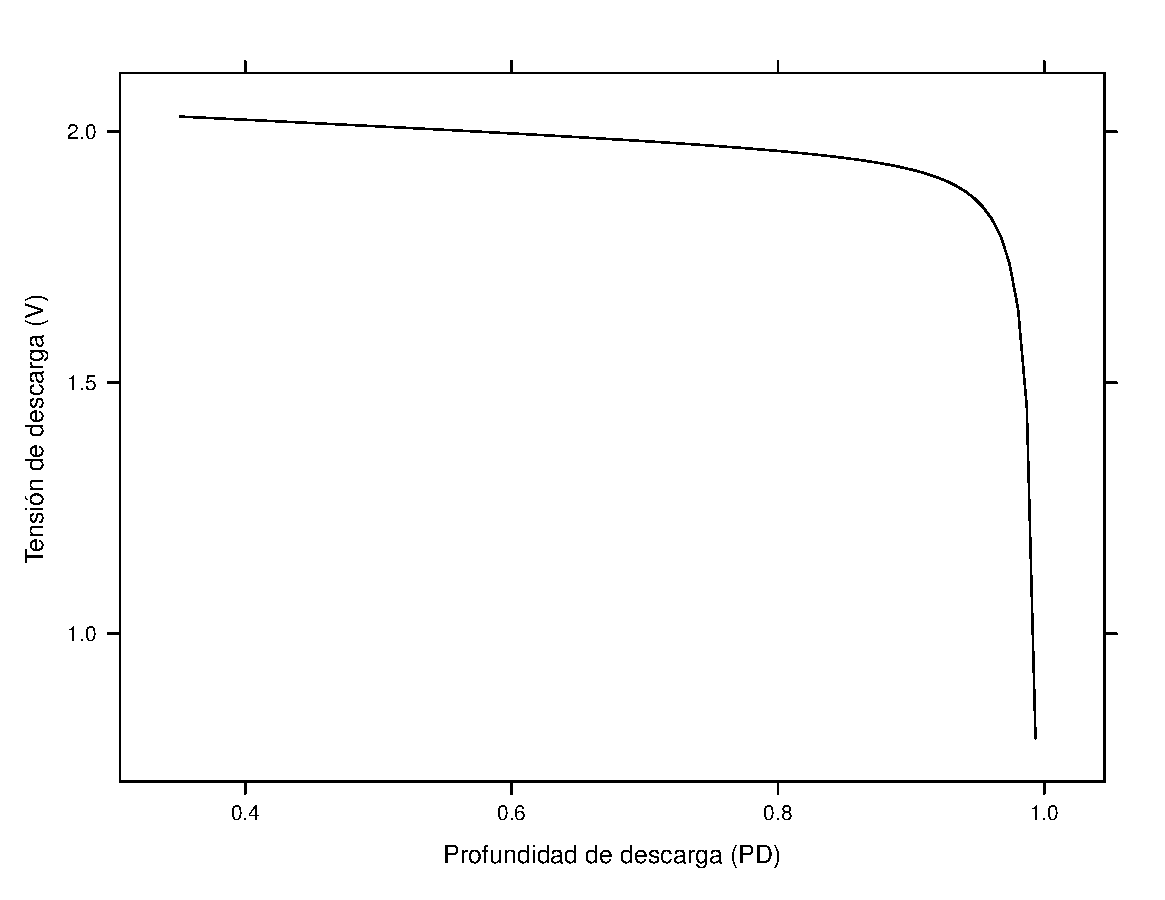
\includegraphics[width=.9\linewidth]{../figs/Bateria_SOCyDescarga.pdf}
\end{frame}

\begin{frame}[label=sec-2-2-6]{Carga}
\begin{itemize}
\item El sulfato de plomo se transforma en oxido de plomo, plomo y acido.

\item Con largos períodos en estados parciales de carga, el ácido se concentra en el fondo por gravedad (\alert{estratificación})

\begin{itemize}
\item Las reacciones no se producen de igual forma en toda la extensión de las placas, lo que realimenta el proceso.

\item Puede reducirse mediante un gaseo controlado.
\end{itemize}

\item Al terminar el proceso de carga se produce la electrolisis del agua, con liberación de oxigeno e hidrógeno (\alert{gaseo}):

\begin{itemize}
\item Pérdida de agua del electrolito (hay que reponerla)

\item Homogeneización del electrolito por agitación (reduce la estratificación)
\end{itemize}
\end{itemize}
\end{frame}


\begin{frame}[label=sec-2-2-7]{Descarga}
\begin{itemize}
\item Ambos electrodos transforman la materia activa en sulfato de plomo en ambos y agua en el ánodo.

\item \alert{Consumo de electrolito} (disminuye su densidad) y \alert{cambios de volumen} de los materiales activos.

\item \alert{Descargas repetidas} producen \alert{pérdida de material activo} y degradación de las placas.

\item Si la descarga es muy rápida y la bateria permanece descarga largo tiempo, el sulfato cristaliza y no es recuperable (\alert{sulfatación}).
\end{itemize}
\end{frame}


\subsection{Efecto de la temperatura}
\label{sec-2-3}

\begin{frame}[label=sec-2-3-1]{Temperatura baja}
\begin{itemize}
\item El electrolito se hace más viscoso y decrece la movilidad de los iones (aumenta la resistencia eléctrica)

\item \alert{Baja la capacidad} para un regimen de descarga determinado a razón de 1\%/ºC

\item Si el electrolito se congela, no hay movimiento iónico, y por tanto la capacidad es nula. Para evitarlo, \alert{hay que recurrir a densidades altas de electrolito en lugares muy frios}.
\end{itemize}
\end{frame}

\begin{frame}[label=sec-2-3-2]{Temperatura alta}
\begin{itemize}
\item \alert{Acelera las reacciones, favoreciendo la corrosión}. Por tanto, decrece la vida de la batería.

\item En \alert{climas cálidos}, se debe optar por \alert{bajas concentraciones de electrolito} (que se ve compensada por la mayor movilidad iónica debida a la alta temperatura).

\item \alert{Baja el valor de tensión al que empieza la sobrecarga} debido a que la resistencia interna baja con la temperatura.

\begin{itemize}
\item Hay que corregir el umbral de corte con la temperatura (se puede utilizar la ambiente como referencia)
\end{itemize}
\end{itemize}
\end{frame}

\begin{frame}[label=sec-2-3-3]{Capacidad según el regimen de descarga y la temperatura}
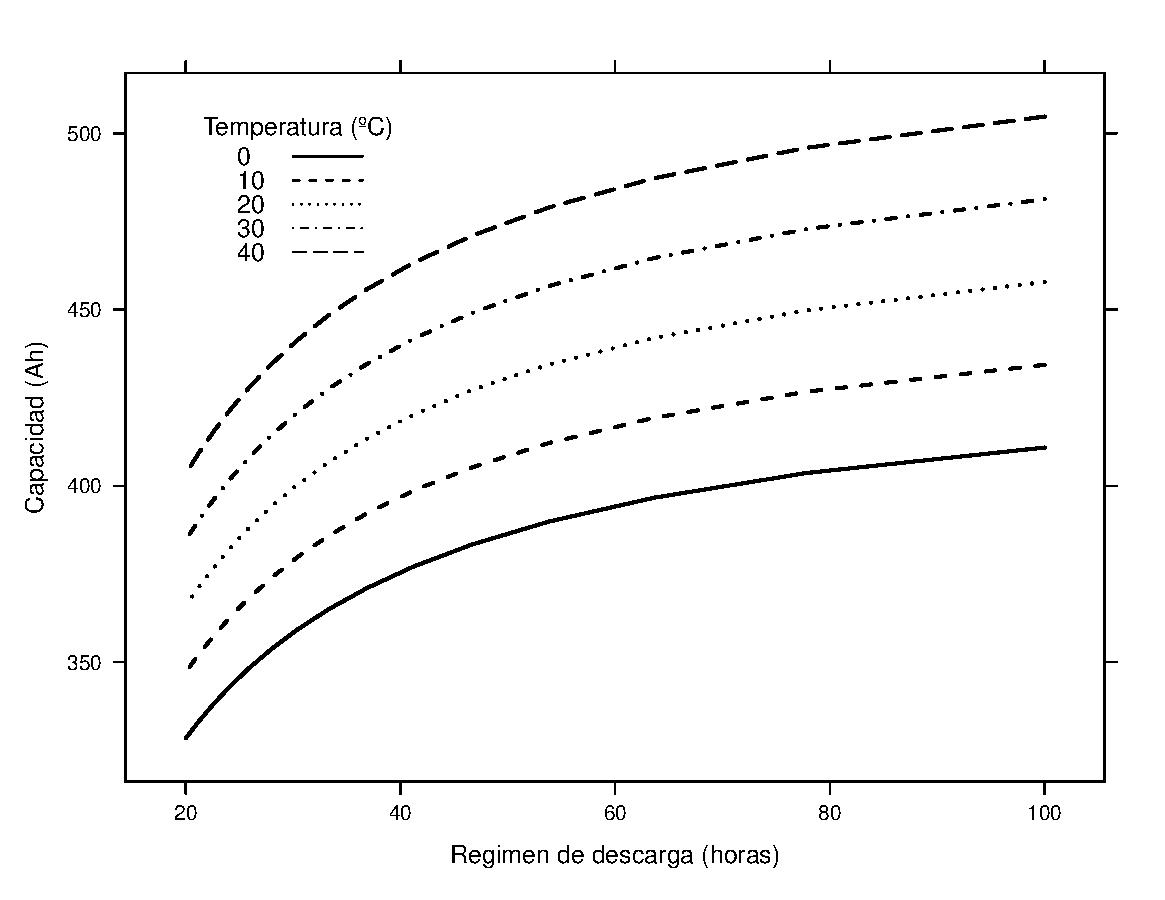
\includegraphics[width=.9\linewidth]{../figs/Bateria_Capacidad.pdf}
\end{frame}

\subsection{Ciclado}
\label{sec-2-4}
\begin{frame}[label=sec-2-4-1]{Definición}
\begin{itemize}
\item \alert{El ciclado es el proceso por el que un acumulador es continuamente cargado y descargado durante su vida.}

\item El ciclado y los agentes externos contribuyen a degradar el acumulador hasta que alcanza el fin de su vida útil, momento que puede ser definido como un valor mínimo en su capacidad útil.
\end{itemize}
\end{frame}

\begin{frame}[label=sec-2-4-2]{Resistencia al ciclado}
\begin{itemize}
\item \alert{La profundidad de descarga}: las descargas profundas disminuyen los ciclos de vida de una batería.

\item \alert{El régimen de carga}: cuanto mayor es el régimen de carga y el porcentaje de sobrecarga, menor será la vida alcanzada.

\item \alert{La temperatura}: las temperaturas altas aceleran la corrosión en los electrodos disminuyendo los ciclos de vida.
\end{itemize}
\end{frame}


\subsection{Composición}
\label{sec-2-5}

\begin{frame}[label=sec-2-5-1]{Composición}
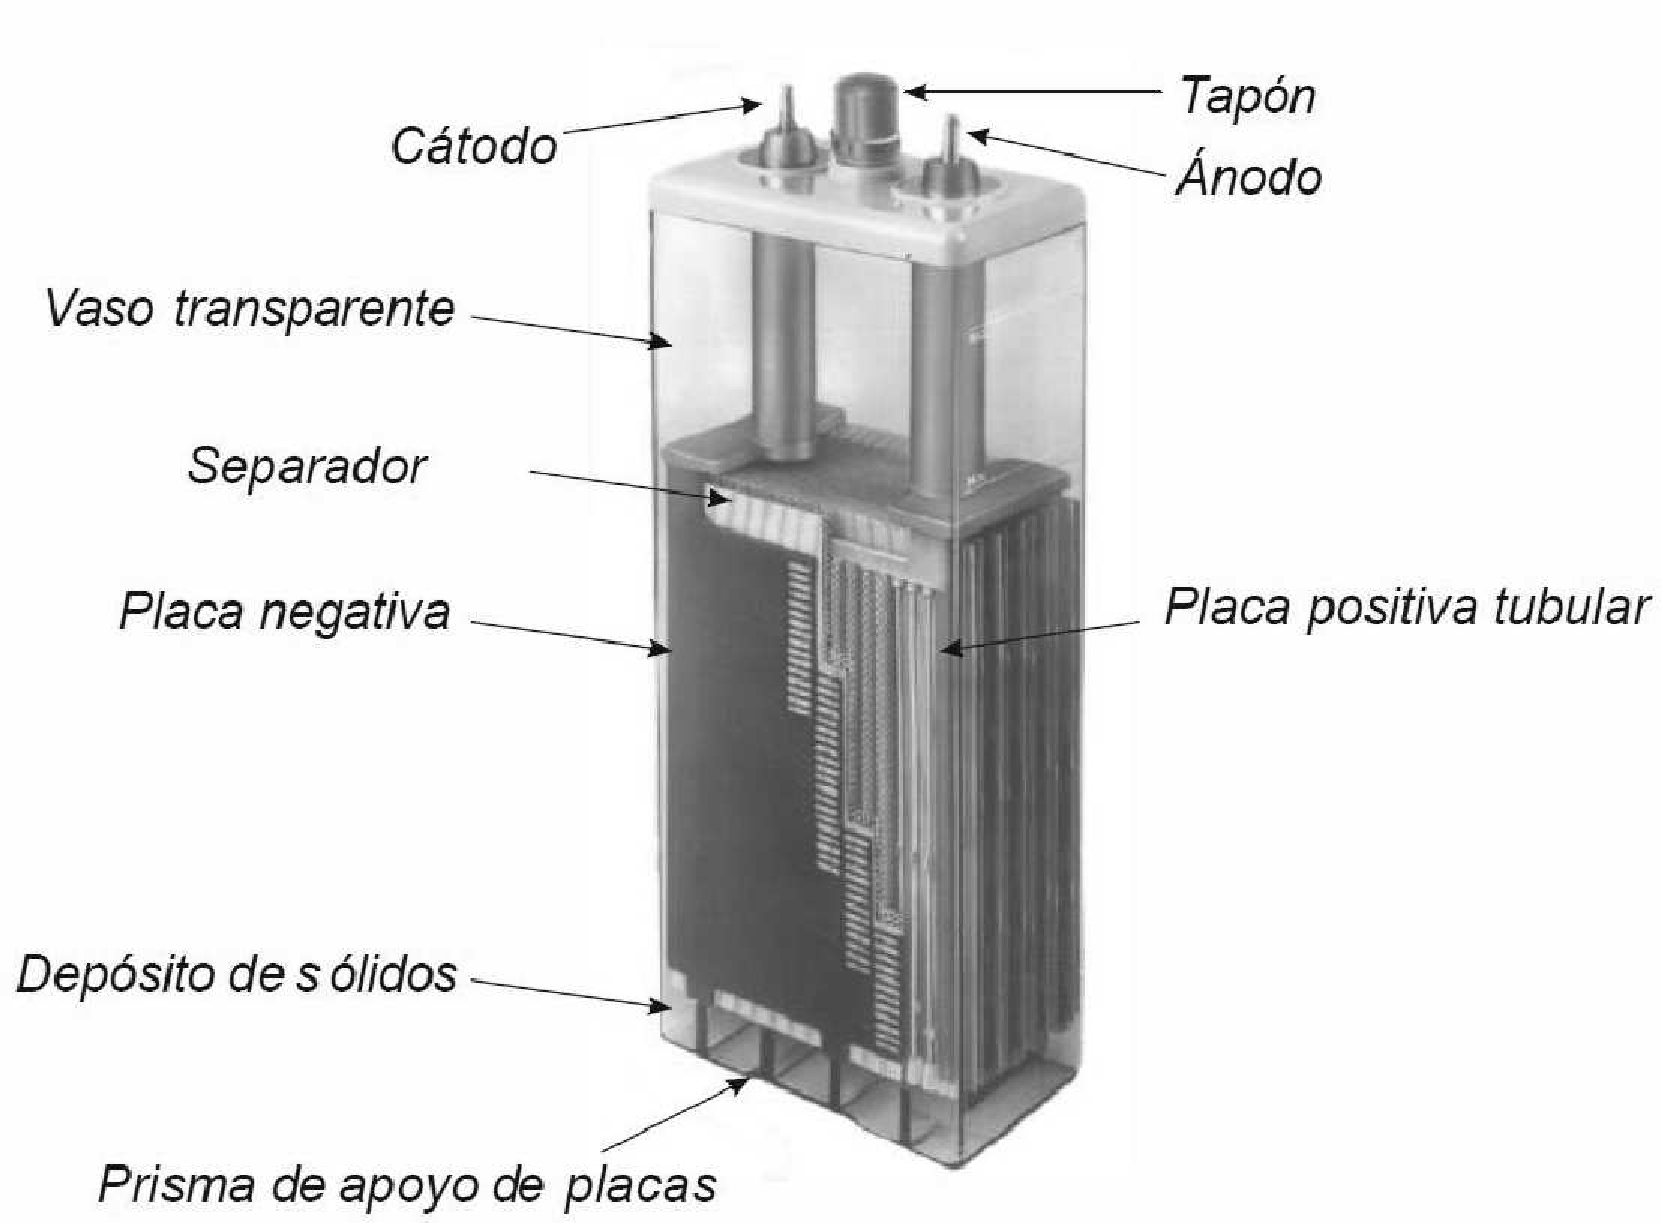
\includegraphics[width=.9\linewidth]{../figs/AcumuladorBN.pdf}
\end{frame}

\begin{frame}[label=sec-2-5-2]{Rejillas}
\begin{itemize}
\item Las rejillas dan \alert{soporte estructural a los materiales activos} (oxido de plomo en ánodo, plomo en cátodo) y \alert{conducen la corriente
eléctrica} hacia el circuito externo.

\item Están fabricadas en \alert{aleaciones de Plomo}.

\begin{itemize}
\item La \alert{aleación de plomo-calcio} proporciona alta resistencia a la corrosión por sobrecarga pero presenta elevada corrosión en bajos
estados de carga.

\item La \alert{aleación de plomo-antimonio} presenta buen comportamiento en ciclado y en descarga profunda.
\end{itemize}

\item \alert{La rejilla negativa es plana}, mientras que la \alert{rejilla positiva puede ser plana} (operación en flotación) \alert{o tubular} (operación en
ciclado).
\end{itemize}
\end{frame}

\begin{frame}[label=sec-2-5-3]{Materiales activos y electrolito}
\begin{itemize}
\item Los materiales activos participan en las reacciones químicas. Están \alert{adheridos a las rejillas}. Deben ser \alert{porosos} para permitir la
penetración del electrolito

\item El \alert{electrolito} participa en la reacción y \alert{realiza el transporte iónico} para cerrar el ciclo de corriente de las reacciones.

\item La \alert{elección del electrolito} debe tener en cuenta su \alert{densidad, conductividad, punto de congelación, poder de corrosión e impurezas}.
\end{itemize}
\end{frame}

\begin{frame}[label=sec-2-5-4]{Electrolito}
\begin{itemize}
\item \alert{Para reducir la resistencia eléctrica del electrolito, su densidad debe ser alta}, pero \alert{un electrolito de alta densidad es muy agresivo} (produce corrosión en la rejilla positiva).

\item Altos regímenes de descarga requieren mayor densidad para facilitar el transporte iónico. Los acumuladores estacionarios utilizan densidades más bajas que los de arranque.

\item El electrolito \alert{puede ser líquido} (aireadas) \alert{o inmovilizado} (selladas).
\end{itemize}
\end{frame}

\begin{frame}[label=sec-2-5-5]{Separadores}
\begin{itemize}
\item Los separadores \alert{aislan las placas de diferente polaridad pero permiten el movimiento iónico a través suyo}. Deben tener resistencia mecánica, ser permeables y porosas, resistentes a la oxidación, sin contaminantes y electricamente no conductores.
\end{itemize}
\end{frame}

\subsection{Tipos de acumuladores}
\label{sec-2-6}

\begin{frame}[label=sec-2-6-1]{Características generales}
\begin{itemize}
\item Un acumulador incorporado a un SFA debe ser \alert{capaz de funcionar sometido a ciclados diarios y anuales de carga y descarga}, teniendo en cuenta que la carga entregada por el generador depende directamente de la radiación (variable en los períodos intradiario e intraanual).

\item Debido a las posibles fluctuaciones en la carga aportada, es probable que se sucedan \alert{periodos prolongados en carga parcial}.

\item Es habitual que las \alert{descargas sean a baja intensidad con periodos de descarga largos}, típicamente en torno a las 100 horas.
\end{itemize}
\end{frame}

\begin{frame}[label=sec-2-6-2]{Baterías de arranque}
\begin{itemize}
\item Habitualmente empleadas en automóviles

\item Fácilmente localizables en cualquier mercado local a bajo precio (relativo)

\item Opción frecuentemente empleada en sistemas de electrificación rural de pequeño tamaño

\item Reemplazo de baterías estropeadas

\item Buen comportamiento en descarga de alta intensidad y tienen buen rendimiento de descarga a bajas temperaturas.

\item No son resistentes frente al ciclado
\end{itemize}
\end{frame}

\begin{frame}[label=sec-2-6-3]{Baterías de tracción}
\begin{itemize}
\item Empleadas, por ejemplo, en carretillas elevadoras.

\item Resistencia suficiente para soportar un elevado número de ciclos profundos de carga-descarga.

\item Requieren aportación de agua y mantenimiento frecuente.

\item Empleo en SFA sólo cuando exista mantenimiento regular.
\end{itemize}
\end{frame}

\begin{frame}[label=sec-2-6-4]{Baterías estacionarias}
\begin{itemize}
\item Empleadas en sistemas de alimentación ininterrumpida (UPS) o instalaciones remotas (por ejemplo, radioenlaces).

\item Funcionan en régimen de flotación.

\item Gran reserva de electrolito aunque realizan poco uso de agua.

\item Resistencia a la corrosión y elevada fiabilidad.

\item Opción muy interesante para SFA. Precio más elevado frente a las anteriores opciones.
\end{itemize}
\end{frame}

\begin{frame}[label=sec-2-6-5]{Baterías \guillemotleft{}fotovoltaicas\guillemotright{}}
\begin{itemize}
\item Baterías SLI modificadas (baratas)

\item Baterías estacionarias modificadas (caras)
\end{itemize}
\end{frame}

\begin{frame}[label=sec-2-6-6]{Elección de batería}
\begin{itemize}
\item La elección entre uno u otro tipo es un ejercicio que debe tener en consideración no sólo \alert{criterios puramente técnicos} sino también aspectos como el \alert{coste del sistema}, recursos de \alert{mantenimiento} disponibles durante la vida del sistema, \alert{disponibilidad de reemplazo} en el mercado local o capacidad de intervención del usuario.

\item No obstante, \alert{para aplicaciones fotovoltaicas se recomienda usar baterías estacionarias aireadas de placa positiva tubular, o al menos baterías SLI modificadas} (placas más gruesas, mayor cantidad de electrolito por encima de las placas, más baratas que las estacionarias), con aleación de Pb-Sb en la rejilla y vaso transparente
\end{itemize}
\end{frame}

\section{Regulador de carga}
\label{sec-3}

\begin{frame}[label=sec-3-0-1]{Definición}
Un regulador de carga es un equipo electronico capaz de \alert{evitar la sobrecarga y la descarga excesiva de un acumulador} desconectando al acumulador del generador o del consumo \alert{cuando se alcanzan determinados estados umbral, generalmente determinados por la tensión en bornes}.
\end{frame}

\begin{frame}[label=sec-3-0-2]{Regulador Serie y paralelo}
\begin{itemize}
\item Regulador Serie
\end{itemize}
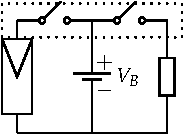
\includegraphics[height=0.3\textheight]{../figs/ReguladorSerie.pdf}

\begin{itemize}
\item Regulador Paralelo
\end{itemize}
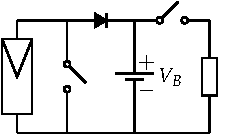
\includegraphics[height=0.3\textheight]{../figs/ReguladorParalelo.pdf}
\end{frame}


\begin{frame}[label=sec-3-0-3]{Ciclo de carga}
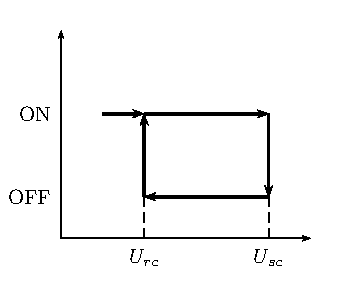
\includegraphics[height=0.5\textheight]{../figs/HisteresisCargaRegulador.pdf}

\begin{itemize}
\item $U_{sc}$ debe estar en el rango de $\SI{2.3}{\volt}$ a $\SI{2.4}{\volt}$ por vaso a $\SI{25}{\celsius}$.

\item $U_{rc}$ debe estar en el rango de $\SI{2.15}{\volt}$ a $\SI{2.2}{\volt}$ por vaso a $\SI{25}{\celsius}$.

\item \alert{Deben corregirse por temperatura} a razón de $\SI{4}{\milli\volt\per\celsius}$ a $\SI{5}{\milli\volt\per\celsius}$ por vaso.
\end{itemize}
\end{frame}

\begin{frame}[label=sec-3-0-4]{Ciclo de descarga}
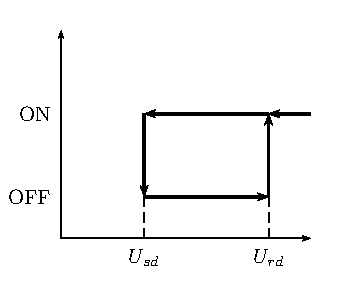
\includegraphics[height=0.5\textheight]{../figs/HisteresisDescargaRegulador.pdf}

Los umbrales deben adaptarse a cada tipo de batería (mediante ensayos, o recomendaciones del fabricante)
\end{frame}

\section{Luminarias}
\label{sec-4}

\begin{frame}[label=sec-4-0-1]{Funcionamiento}
\begin{itemize}
\item Una lámpara fluorescente convencional está formada por un \alert{tubo de descarga con gas a baja presión}, un \alert{recubrimiento de una mezcla de polvos fluorescentes} y \alert{dos electrodos} en los extremos.

\item Un \alert{circuito auxiliar (balasto)} cumple dos funciones principales:

\begin{itemize}
\item \alert{Proporciona la tensión de encendido} necesaria para que fluya corriente por el tubo.

\item \alert{Regula la corriente} que circula por el tubo una vez que se ha producido el encendido para evitar su destrucción.
\end{itemize}
\end{itemize}
\end{frame}

\begin{frame}[label=sec-4-0-2]{Fotometría}
\begin{description}
\item[{Flujo}] radiante es la potencia emitida por la fuente luminosa (Unidad: Watio)

\item[{Flujo}] luminoso es la potencia emitida capaz de producir sensación luminosa en el ojo humano (Unidad: Lumen)

\item[{Iluminación}] de una superficie sobre la que incide un flujo luminoso es el ratio entre flujo y superficie (Unidad: lux, $\si{\lumen\per\watt\squared}$).

\item[{Eficiencia}] de la luminaria (tubo y balasto) es la relación entre potencia eléctrica consumida por el conjunto y la potencia luminosa producida (Unidad: $\si{\lumen\per\watt}$).
\end{description}
\end{frame}
\begin{frame}[label=sec-4-0-3]{Degradación}
\begin{itemize}
\item \alert{El proceso de encendido es el que más contribuye a la degradación} de los tubos fluorescentes.
\item Un método alternativo consiste en \alert{precalentar los electrodos} (con un circuito basado en un condensador y en una resistencia) facilitando el paso a la etapa de emisión termoiónica, y acortando el período de encencedido.
\end{itemize}
\end{frame}

\begin{frame}[label=sec-4-0-4]{Requisitos}
\begin{itemize}
\item Recomendable eficiencia superior a 50 $\si{\lumen\per\watt}$

\begin{itemize}
\item \alert{Debe ser superior a 35 $\si{\lumen\per\watt}$}.
\end{itemize}

\item Recomendable resistencia a un mínimo de 10000 ciclos de encendido y apagado

\begin{itemize}
\item \alert{Deberá resistir 5000 ciclos.}
\end{itemize}
\end{itemize}
\end{frame}
% Emacs 24.4.1 (Org mode 8.2.7c)
\end{document}